
\section{Transcritical flow with a shock over a bump}

This scenario simulates a transcritical flow over a bump with a shock. The topography and the initial conditions are the same as those used in the subcritical flow (See the description given in the report on the subcritical flow test). However, to get a transcritical flow, the boundary conditions are different from those used in the subcritical flow test. Here we refer to the parameters used by Goutal and Maurel~\cite{GM1997}.

Referring to our description for the subcritical flow test, the analytical height or depth $h$ of the transcritical flow at smooth regions is found by solving the Bernoulli equation. The analytical solution for the shock position is found by implementing three equations, namely, (a) the Bernoulli equation at upstream (on the left of the shock), (b) the Bernoulli equation at downstream (on the right of the shock), and (c) the Rankine-Hugoniot relation. The Rankine-Hugoniot relation for the steady flow can be expressed as
\begin{equation}
q^2 \left( \frac{1}{h_1} - \frac{1}{h_2} \right) + \frac{g}{2} \left(h_1^2 - h_2^2\right) = 0\,,
\end{equation}
where $q$ is the discharge or momentum, $h_1$ is the height upstream (on the left of the shock), and $h_2$ is the height downstream (on the right of the shock). When the height $h$ has been found, the velocity is computed as $u=q/h$\,.

\subsection{Results}
For our simulation, we consider Dirichlet boundary conditions
at $x=0^{-}$ given by
\begin{equation}
[w,hu,hv]=[0.41373588752426715,~~~0.18,~~~0]\,,
\end{equation}
and at $25^{+}$ given by
\begin{equation}
[w,hu,hv]=[0.33,~~~0.18,~~~0]\,.
\end{equation}
With these conditions, representatives of the simulation results are shown in the following three figures. They show the stage, $x$-momentum, and $x$-velocity respectively. We should see good agreement between the analytical and numerical solutions.

\begin{figure}
\begin{center}
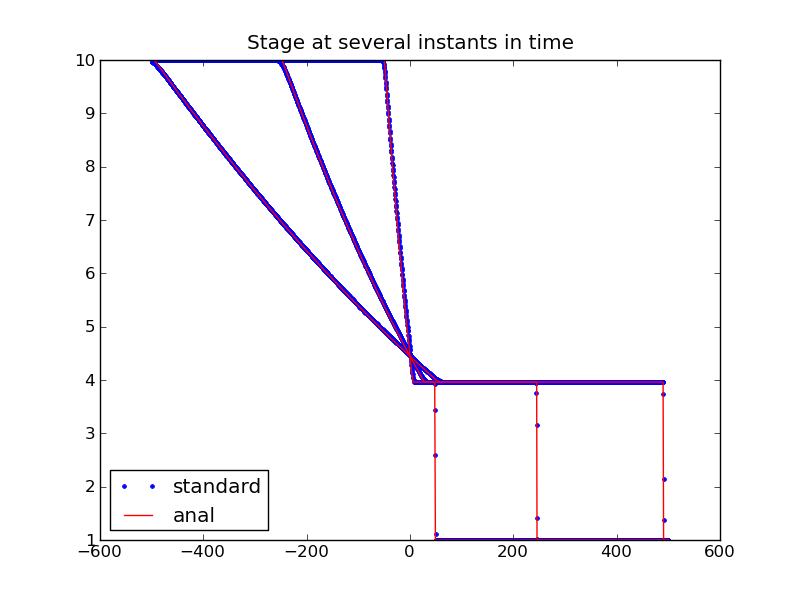
\includegraphics[width=0.9\textwidth]{stage_plot.png}
\end{center}
\caption{Stage results}
\end{figure}


\begin{figure}
\begin{center}
\includegraphics[width=0.9\textwidth]{xmom_plot.png}
\end{center}
\caption{Xmomentum results}
\end{figure}


\begin{figure}
\begin{center}
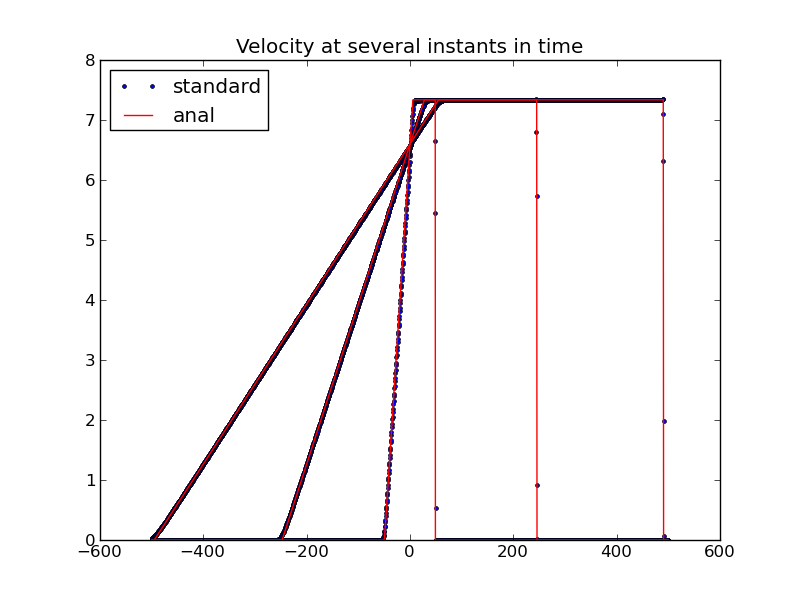
\includegraphics[width=0.9\textwidth]{xvel_plot.png}
\end{center}
\caption{Xvelocity results}
\end{figure}


\endinput
